\documentclass[journal]{IEEEtrancz}
% zvolte kodovani
\usepackage[utf8]{inputenc} % linux/unix
%\usepackage[latin2]{inputenc}
%\usepackage[cp1250]{inputenc} % Windows
\usepackage[czech]{babel}
\usepackage{graphicx}
\usepackage{multirow}
\usepackage{booktabs}

\newcommand{\Cpp}{C\raisebox{0.15ex}[0ex][0ex]{++}}

\begin{document}

\title{Užití GO pro optimalizaci designu molekul ve 2D}
\author{Ladislav Horký}

\maketitle

\begin{abstrakt}
Cílem práce bylo naprogramovat algoritmus genetické optimalizace pro minimalizaci napětí vazeb v 2D molekule s pevně zadanými meziatomárními vzdálenostmi některých atomů. Pro zjednodušení výpočtů byly pozice atomů reprezentovány pouze na celočíselné mřížce, vzdálenosti byly desetinné. Jako testovací molekuly byly zvoleny 22-atomová podlouhlá hexagonální mříž a 49-atomová plně propojená molekula. Zatímco u sítě se často projevovaly typické jevy jako překroucení a zaseknutí se v LO, plně propojená molekula potřebovala k dosažení stavu blízkému globálnímu optimu stabilně zhruba 400-600 generací.

%Zde uvést krátky odstavec s abstraktem. V abstraktu stručně shrnuto o čem článek je.
%Čtenář je motivován, proč by měl článek číst, poslední věta zpravidla.
%shrnuje dosažené výsledky.
\end{abstrakt}

\IEEEpeerreviewmaketitle

\section{Zadání}
Implementovat v \Cpp  genetický algoritmus pro optimalizaci napětí v 2D molekule způsobené nedodržením meziatomárních vazeb (nemusí být zadané mezi všemi atomy). Zaměřit se na operátory mutace a křížení a experimentovat s nimi.

%Několika větami naformulované zadání práce tak, jak jste je dohodli se cvičicím.

\section{Popis algoritmu}
Zde popíšeme stavební kameny algoritmu.

\subsection{Reprezentace jedince}
Molekula o $n$ atomech je reprezentována jako $2n$-složkový vektor typu signed int (32 bitů), obsahující pozice jednotlivých atomů na celočíselné mřížce -- jedná se tedy o celočíselnou optimalizaci. Složky vektoru jsou řazeny po celých atomech,  $(x_1,y_1,x_2,y_2,...,x_n,y_n)$.

\subsection{Selekce}
Pro větší modularitu programu je selekce jedinců pro křížení řešena odděleně pomocí mating pool. Vzhledem k tomu, že v našem případě jsou pro křížení potřeba pouze dva rodiče, je velikost mating pool dvojnásobkem velikosti potomstva. V programu je mating pool reprezentován jednoduše polem ukazatelů do populace.

Jako selekční algoritmus byl zvolen 2-tournament: vybereme náhodně dva jedince z populace a toho s lepší fitness dáme do mating pool. Výhoda tohoto postupu oproti ruletovému kolu je, že se jedná o selekci založenou pouze na pořadí jedinců (podle fitness) a je tedy méně citlivá na nevhodné rozdělení fitness v populaci. Navíc, i když je založená na pořadí, nepotřebuje žádné třídění a je teoreticky velmi dobře paralelizovatelná.

\subsection{Reprodukce}
Nový potomek vznikne vždy z dvojice jedinců z mating pool pomocí $k$-bodového křížení, přičemž možné body křížení jsou omezeny pouze na celé atomy -- nemůže se tedy stát že potomek bude mít $x_1$ z prvního rodiče a $y_1$ z druhého. V programu je skutečný počet bodů křížení náhodný, a to z intervalu $[1,k]$, kde $k$ je stanovená horní hranice. Dále je možno u křížení nastavit míru parazitismu. Místo druhého rodiče z mating pool je pak pro křížení vygenerován náhodný jedinec, jehož žádná souřadnice však v absolutní hodnotě nepřesáhne maximum absolutních hodnot souřadnic prvního rodiče.

\subsection{Mutace}
Po vytvoření potomků křížením jsou tito s danou pravděpodobností zmutováni. Nejprve je vygenerován náhodný bod s rozdělením $N_2(\mathbf{0},\sigma^2)$, kde $\sigma$ je zvolená konstanta. Tento bod je pak přičten k náhodnému počtu bodů (opět z intervalu $[1,k]$, kde $k$ je zvolená konstanta).

Součástí mutace je i následné vycentrování všech potomků, aby jejich těžiště leželo na souřadnicích $(0,0)$, a následné náhodné natočení (opět všech) potomků o náhodný úhel s normálním rozdělením. Diskuse těchto kroků viz dále.

\subsection{Ohodnocení}
Výpočet fitness u potomků je prováděn následovně: vzdálenosti atomů v molekule jsou zadány pomocí symetrické nezáporné matice, kde $A_{ij}$ udává vzdálenost $i$-tého a $j$-tého atomu. Pokud je prvek matice nulový, znamená to, že na vzdálenosti daných atomů nezáleží. Fitness jedince je pak dána sumou rozdílů předepsaných a skutečných vzdáleností mezi atomy (pouze tam, kde je $A_{ij}$ nenulové).

V průběhu ohodnocení je prováděn i základní niching tak, že z jedinců, kteří se alespoň v jedné souřadnici neliší o více než zvolenou konstantu (v našem případě 5), je ponechán pouze jediný (ostatním je násobně zvýšena fitness).

\subsection{Vytvoření nové populace}
Po ohodnocení potomků vybereme nejprve ze staré populace nastavený počet elitních jedinců s nejnižší fitness. Ti jsou poté doplněni do počtu původní populace nejlepšími jedinci z potomstva.

\section{Implementační poznámky}
Program je napsán \Cpp  za vydatného použití šablon. Hlavním objektem je \textit{populace}, s metodami \textit{Create} a \textit{GetNextGeneration}, které obstarávají celý běh algoritmu. Způsob reprodukce, mutace, ohodnocení, selekce a míšení staré a nové populace se \textit{populaci} předávají jako šablonové parametry a konkrétní algoritmus (nejen) genetické optimalizace je tak možné poskládat z velmi jednoduchých stavebních bloků.

\section{Experimentální výsledky}
Provedl jsem měření rychlosti konvergence u 22- i 49-atomové molekuly, u 49-atomové molekuly byl navíc pozorovnám vliv vycentrování a otočení jedince na průběh optimalizace. Všechny experimenty měly stejné parametry populace, a to 60 jedinců v populaci a 1500 v potomstvu.

22-atomová molekula měla tvar podlouhlé pravidelné hexagonální sítě s hranou délky 200. 49-atomová molekula měla tvar smajlíka nakresleného na ortogonální mřížce s hranou 100, jeho průměr byl 1500. Tato molekula byla na rozdíl od první zcela propojená, což zaručovalo existenci pouze jednoho (až na natočení) globálního optima.
\begin{figure}[h]
        \begin{minipage}[l]{0.22\textwidth}
            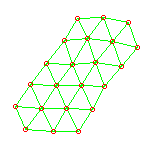
\includegraphics[width = 80pt]{globopt.png}
            \caption{22-atomová}
        \end{minipage}
        \begin{minipage}[r]{0.22\textwidth}
            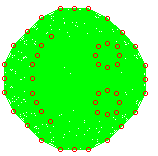
\includegraphics[width = 80pt]{smajl.png}
            \caption{49-atomová}
        \end{minipage}
\end{figure}

\subsection{Rychlost konvergence}
Měření bylo prováděno na 100 bězích algoritmu. Maximální počet bodů křížení byl u obou molekul nastaven na 20, míra parazitismu na 10\% a počet elitních jedinců na 3. Rozptyl mutace, míra mutace a počet bodů mutace byly u 49-atomové molekuly nastaveny na 20,30\%,5, u 22-atomové pak na 30,40\%,10.

Nejlepší případy uvádí tabulka \ref{tab:besconv}. Konvergenci algoritmu jsem definoval jako okamžik, kdy nebyl během posledních 20 (resp. 100 v případě 22-atomové molekuly) generacích nalezen lepší jedinec.

\begin{table}[h]
  \centering
  \caption{Nejlepší výsledky podle fitness}
  \begin{tabular}{cccc}
  \toprule
   \# atomů & fitness & \# generací & čas \\
  \midrule
  22 & 61.3 & 2635 & 77.2s\\
  49 & 754.7 & 547 & 69.7s\\
  \bottomrule
  \end{tabular}
  \label{tab:besconv}
\end{table}

Nenulové nejlepší fitness jsou dány tím, že atomy jsou usazeny v celočíselné mřížce a zadané vzdálenosti jsou napočítány na 2 desetinná místa. Navíc v případě celočíselné mřížky je fitness závislá i na natočení molekuly. Díky tomu považuji fitness menší než počet vazeb v molekule (a tedy počet zaokrouhlení vlivem mřížky) za velmi dobrou -- ve většině případů se pak opravdu jedná jen o natočené globální optimum.

Průměrné případy se směrodatnou odchylkou a mediánem jsou uvedeny v tabulce \ref{tab:avgconv}. 

\begin{table}[h]
  \centering
  \caption{Průměrné výsledky se směrodatnou odchylkou}
  \begin{tabular}{cccc}
  \toprule
   \# atomů & fitness & \# generací & čas \\
   & \multicolumn{3}{c}{směrodatná odchylka}\\
   & \multicolumn{3}{c}{medián}\\
  \midrule
  \multirow{3}{*}{22} & 3290 & 1058 & 36s\\
                      & 4350 & 868 & 32.3s\\
                      & 1127 & 726 & 23.9s \\
  \multirow{3}{*}{49} & 11623 & 439 & 54.2s\\
                      & 19287 & 165 & 21.7s\\
                      & 1324  & 445 & 54.7s\\
  \bottomrule
  \end{tabular}
  \label{tab:avgconv}
\end{table}

Obecně se dá říci, že 49-atomová molekula se optimalizovala lépe, což je vidět i na malém rozdílu nejlepší a mediánové fitness. Je to dáno tím, že její fitness má ve všech bodech velký gradient a lokální minima jsou relativně mělká -- při pokusech s delšími běhy bez kritéria konvergence molekula ve většině případů dokovnergovala do globálního minima před dosažením 1000. generace.

Naproti tomu u 22-atomové se projevila malá provázanost atomů - fitness měla velké množství hlubokých globálních a lokální optim (typické pro optimalizaci sítí) oddělených oblastmi s malou gradientní informací -- příklad jedince z této oblasti můžeme vidět na obrázku \ref{obr:grad}. Kvůli malému gradientu bylo nutné výše zmíněné zpřísnění konvergenčního kritéria.

\begin{figure}[h]
        \begin{minipage}[l]{0.22\textwidth}
            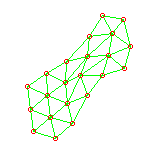
\includegraphics[width = 80pt]{lokmin.png}
            \caption{Malý gradient}
            \label{obr:grad}
        \end{minipage}
        \begin{minipage}[r]{0.22\textwidth}
            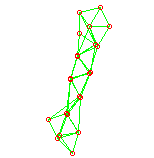
\includegraphics[width = 80pt]{prehnute.png}
            \caption{Přehnutí sítě}  
        \end{minipage}
\end{figure}


\subsection{Vliv operátoru mutace}
V dalším experimentu jsem zkoušel odstranit jednotlivé části mutace (ostatní parametry algoritmu zůstaly zachovány) u 49-atomové molekuly. Následující graf ukazuje typický průběh optimalizace s mutací obsahující pouze přičtení gaussovského šumu (zelená čára), šum + vycentrování (červená čára) a šum + vycentrování + náhodné pootočení (modrá čára).

\begin{figure}[h]
    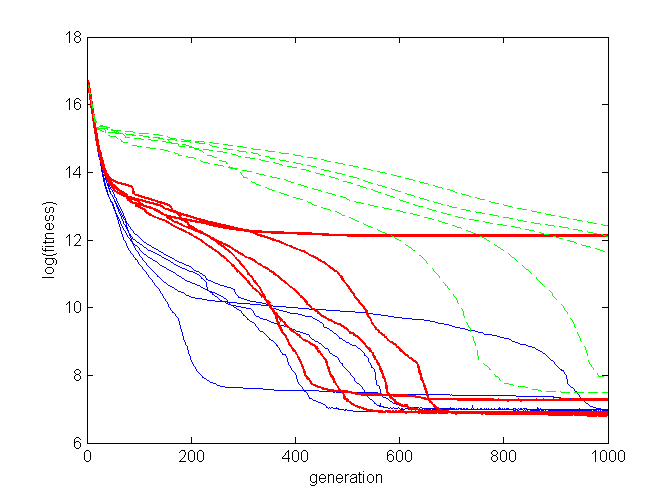
\includegraphics[width = 0.48\textwidth]{vse.png}
    \caption{Srovnání různých operátorů mutace}
\end{figure}

Vidíme, že v první fázi optimalizace funguje hlavně křížení. Pokud neděláme vycentrování po každé generaci, velmi rychle se nám v populaci vytvoří několik stejně kvalitních, navzájem pouze posunutých jedinců -- další kvalitní jedinci pak mohou vzniknout už jen křížením a mutací uvnitř těchto skupin, takže se algoritmus vlastně rozpadne na několik menších, pracujících s menší populací a řádově menším potomstvem (meziskupinoví kříženci jsou stabilně nekvalitní a v potomstvu jen zabírají místo). Tento efekt můžeme vidět na brzkém zlomu zelených grafů, kdy optimalizace skokově několikanásobně zpomalí.

Po vycentrování již funguje algoritmus relativně dobře (technicky vzato ubereme množině globálních optim dva stupně volnosti). Pokud ovšem ještě náhodně každého jedince zrotujeme (což virtuálně nemění jeho fitness), získáme v populaci o trochu větší diverzitu a křížení se uplatní ještě o něco lépe a déle. Navíc, v poslední fázi může rotace pomoci molekule lepšímu usazení do celočíselné mřížky a tak zlepšit výslednou fitness.


\section{Závěr}
Ukázalo se, že pro velmi provázané molekuly funguje algoritmus velmi dobře a díky programování pomocí šablon je i slušně rychlý. Pro málo provázané molekuly však nedokáže uniknout z některých lokálních optim a konvergence je obecně pomalejší. Tyto problémy by se daly řešit komplikovanějším nichingem (který je ale časově značně náročný), který by udržel větší diverzitu v populaci, a -- v případě oblastí s nízkým gradientem -- sofistikovanějším operátorem mutace, který by například pracoval s propojenými celky v molekule, spíše než z jednotlivými atomy. Většina těchto úprav je však již závislá na konkrétním zadání molekuly, a proto jsem se do nich v rámci zachování obecnosti nepouštěl.

\end{document}
